\section{Problem Statement}
\label{sec:problemStatement}

\begin{figure}[t]
\centering
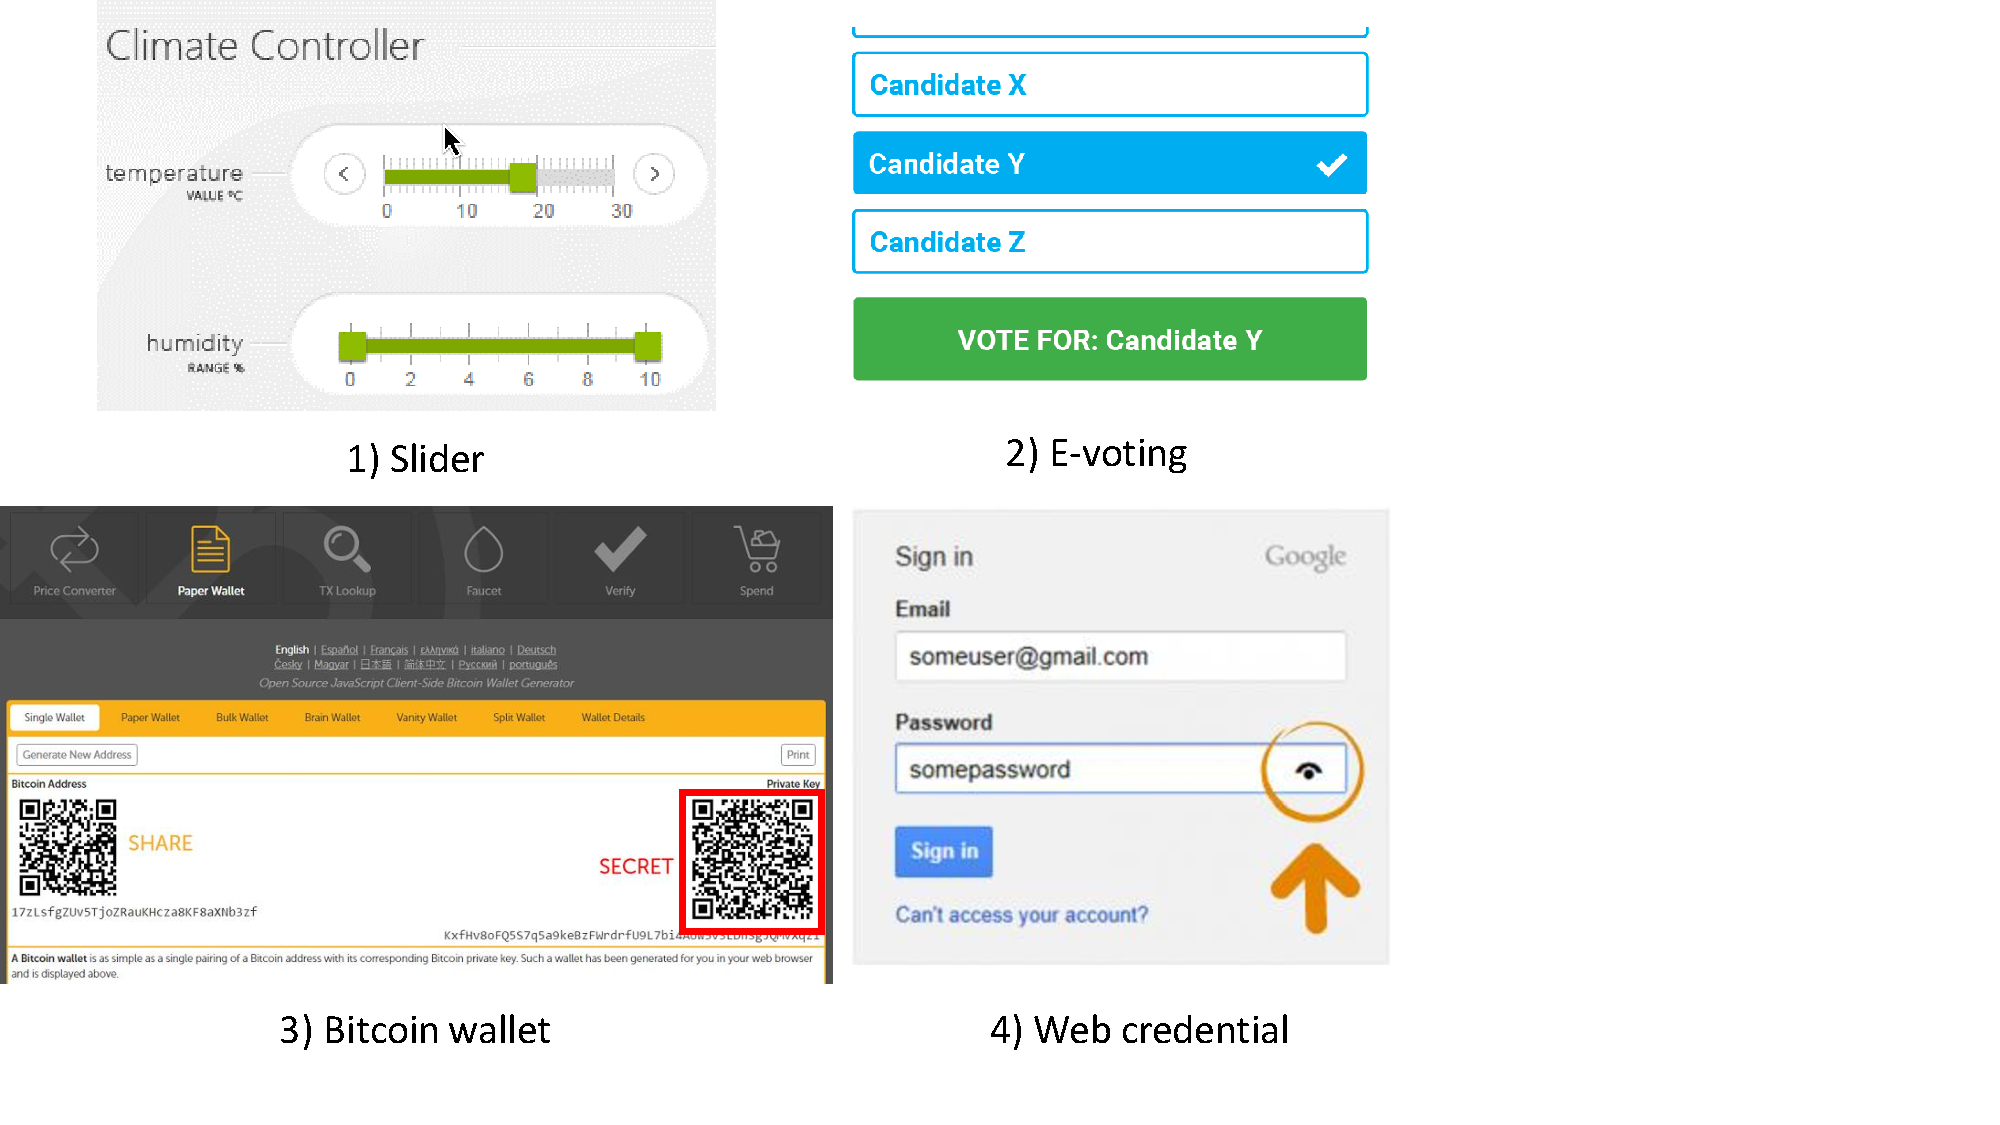
\includegraphics[trim={0 1cm 10cm 0}, clip, width=\linewidth]{motivation.pdf}
\caption{\textbf{Motivating examples.} 1) Pointer based UI elements that sets parameters to remote safety-critical device, 2) E-voting where the voting privacy and integrity is critical, 3) Financial transactions such as bitcoin wallet that shows sensitive information such as the user's private key and 4) web applications that provide an option for the user to reveal credentials.}
\label{fig:motivation}
\centering
\end{figure}



\subsection{Motivation and Problem Statement}

Integrity and privacy of IO data between the user and a sensitive service is a crucial problem when one assumes that the attacker compromises host systems that include the hardware, the operating systems, and all the installed applications. Such an attacker model allows it not only to steal the sensitive information from the user but also alter them. Furthermore, the user is completely unprotected, she cannot verify that her inputs are transferred to the server securely, or even have the guarantee that she is communicating with the legitimate server. 

\myparagraph{Trusted path} is the property that provides the security properties (privacy and integrity) to the IO data between the users and the end systems. In principle trusted path solves the problem of the security of the IO data. But practically establishing a trusted path in general IO devices is a nontrivial problem specifically if one considers the plethora of complex UI objects and input methods.

We list the security properties that we want to provide in our proposed solution. We now discuss these security properties and corresponds them with the motivating example.

\begin{enumerate}
  \item \textbf{Input integrity and privacy.} These properties define that any input that is coming from the user input devices are fully protected in two ways: i) the inputs are that issued by the user reaches to the remote end-point as it was meant to be - \emph{integrity}, and ii) in specific application scenarios, the attacker-controlled host is entirely oblivious about the input from the user - \emph{privacy}. We can further fine grain the user input to the granularity of user-issued \emph{commands} and user-issued \emph{activities}. Both of which are generated by the input devices from the user. User-issued commands are the specific actions that are executed by the user. Commands are transmitted to the remote end-system, e.g., filling a text-box with a parameter and clicking the \emph{submit} button issues a \texttt{HTTP} request to the remote server. The user-issued activities are actions that are given to the host system which are not directly transmitted to the remote end-system but causes user-issued commands, e.g., mouse movement from one point to a button that user intends to click.  
  \item \textbf{Output integrity and privacy.} 
  \end{enumerate}

\begin{figure}[t]
\centering
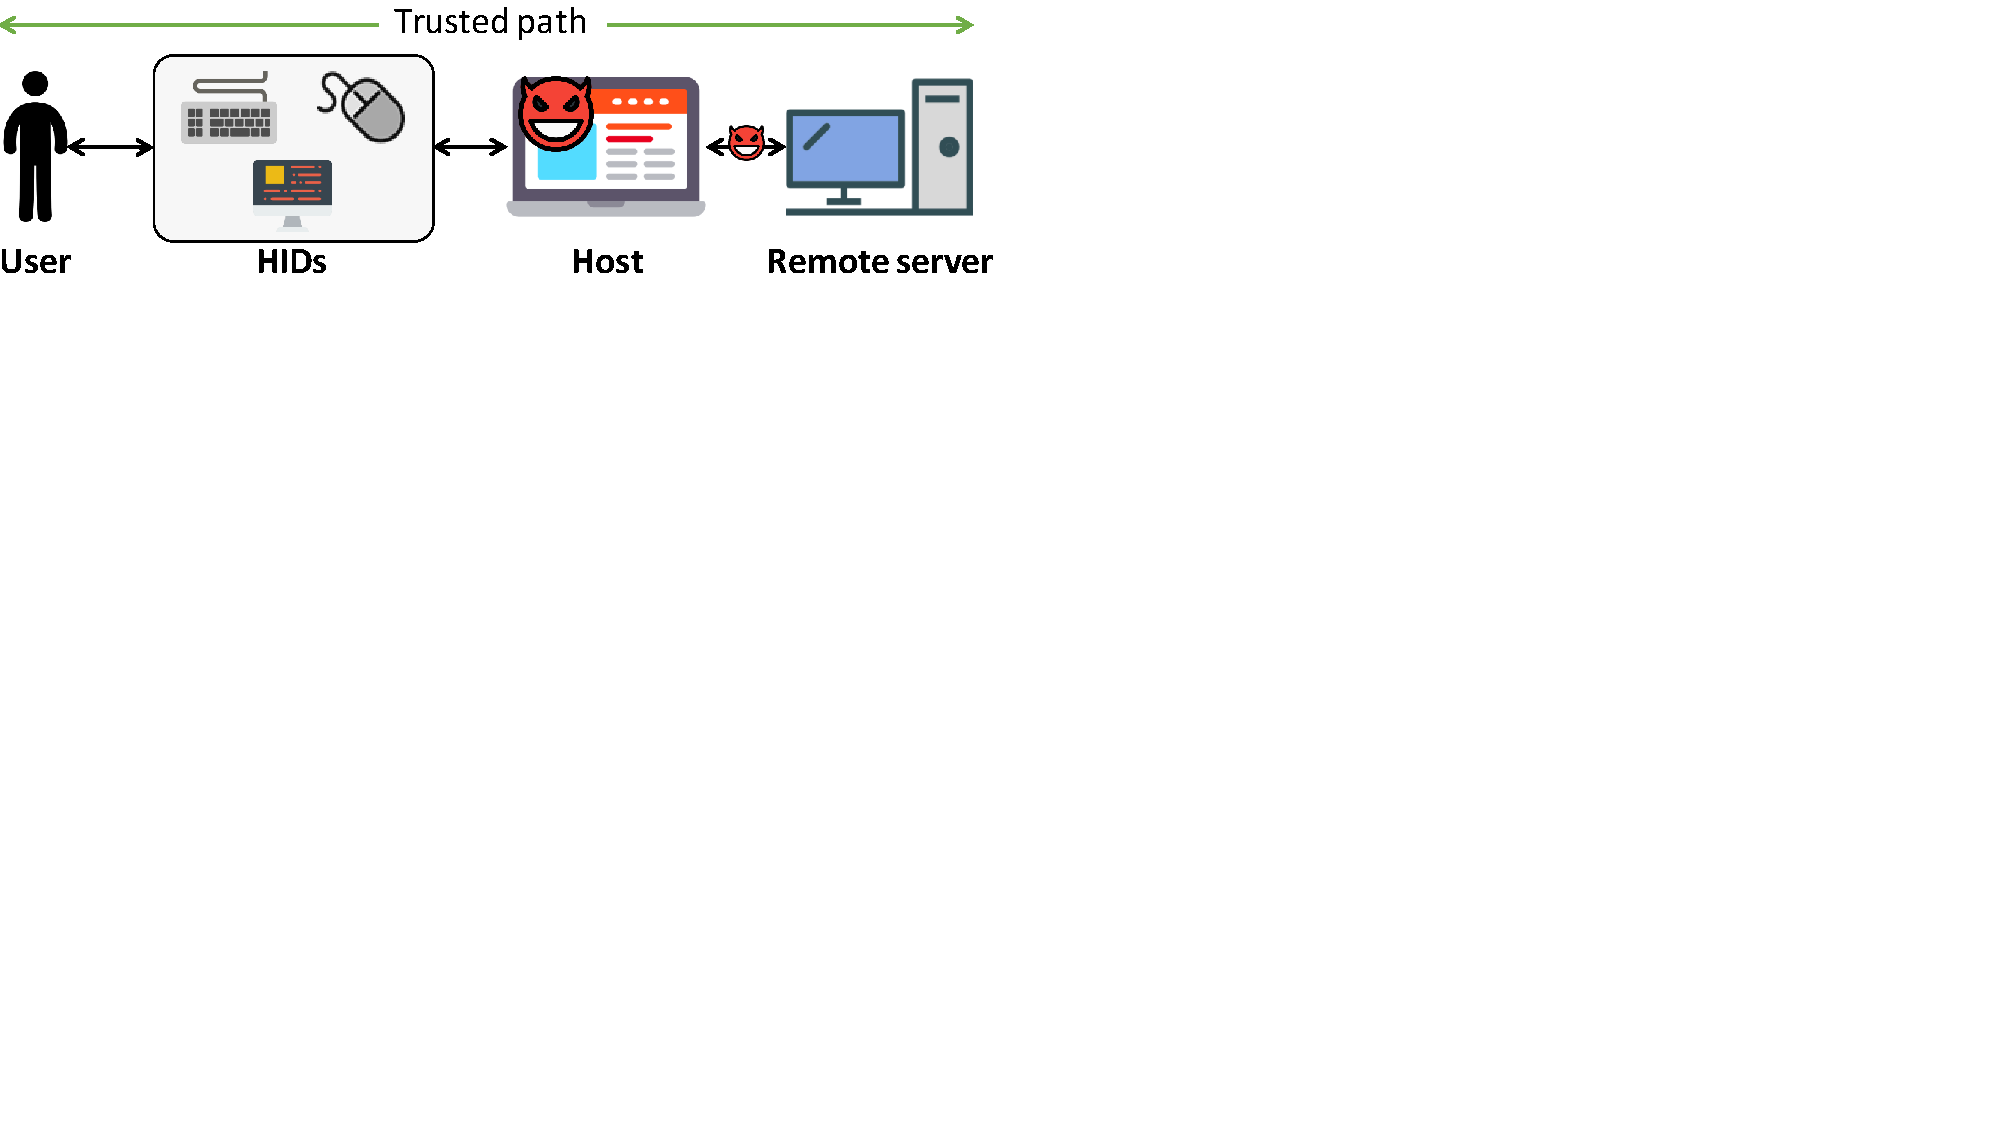
\includegraphics[trim={0 14cm 17cm 0}, clip, width=0.9\linewidth]{systemModel.pdf}
\caption{\textbf{Trusted path system model.} The figures shows the system and the attacker model of the trusted path.}
\label{fig:systemModel}
\centering
\end{figure}

\iffalse
\myparagraph{Advantages}

\begin{enumerate}
  \item The \device does not need to know the formatting/template of the page. As the \device only looks to the current mouse position, the structure of the page is somewhat irrelevant (?).
\end{enumerate}
\fi


\begin{table*}[t]
\centering
  \begin{tabular}{ | l | c | c |}
    \hline
     & TEE & no TEE \\ \hline
    \multirow{6}{*}{Hypervisor based} & SGX IO~\cite{weiser2017sgxio} & Overshadow~\cite{Overshadow} \\ 
    & & Virtual ghost~\cite{criswell2014virtual}\\ 
    & & Inktag~\cite{hofmann2013inktag}\\ 
    & & TrustVisor~\cite{mccune2010trustvisor} \\ 
    & & Splitting interfaces~\cite{ta2006splitting}\\ 
    & & $SP^3$~\cite{yang2008using}\\ \hline
   \multirow{2}{*}{Isolated execution of APIs/Drivers} & BASTION-SGX~\cite{BASTION-SGX} & Slice~\cite{azab2011sice}\\ 
    & TrustOTP~\cite{sun2015trustotp} & CARMA~\cite{vasudevan2012carma} \\ \hline
    \multirow{3}{*}{External trusted hardware based} & Fidelius~\cite{Fidelius} & IntegriKey~\cite{IntegriKey} \\
    &  & FPGA-based~\cite{brandon2017trusted} \\
    &  & \textcolor{OliveGreen}{Our Solution (I + O + Activity)} \\
    \hline
  \end{tabular}
  \caption{Summarization of existing trusted path solutions. Note that in the table, switching systems from left to right or top to bottom, reduces the trust assumption. For example, TEE based solutions, such as SGX-based trusted path solution requires trust on the physical processor packages, SGX APIs, quoting and launch enclaves and Intel attestation service.}
\end{table*}


\subsection{Potential Solutions and their drawbacks}

Given the attacker's model, there exist several solutions that solve the problem of a trusted path to and from the IO devices in the presence of a compromised host. But all of these solutions targeted for different problem settings and models:

\subsubsection{Strawman solution: trusted OS} Trusted OS could be seen as a straightforward solution as traditionally OS handles all the IO drives, computation, and network communications. Assuming a trusted OS significantly reduces the complexity of the solution but the security assumption suffers. Trusted OS introduces a large trusted code base and a multitude of vulnerabilities. 

\subsubsection{Hypervisor-based solutions} Trusted hypervisors and secure micro-kernels are also choices for contrasting Trusted path. Sel4~\cite{klein2009sel4} is a functional hypervisor that is formally verified and has a kernel size of only $8400$ lines of code. In the work done by Zhou et al.~\cite{zhou2012building}, the authors proposed a generic trusted path on $x86$ systems in a pure hypervisor-based design. Examples of other hypervisor based works can be found in systems such as Overshadow~\cite{Overshadow}, Virtual ghost~\cite{criswell2014virtual}, Inktag~\cite{hofmann2013inktag}, TrustVisor~\cite{mccune2010trustvisor}, Splitting interfaces~\cite{ta2006splitting}, $SP^3$~\cite{yang2008using}, etc.

\myparagraph{Trusted Execution Environments} TEEs are another ways to implement a trusted path between the IO devices and the users. Several TEEs such as Intel SGX, ARM TrustZone, TPM, Intel TXT, etc. can be used to achieve such functionality. Previous research works such as Intel SGX and trusted hypervisor-based SGXIO~\cite{weiser2017sgxio}, Intel SGX based ProximiTEE~\cite{dhar2018proximitee}, TPM and TXT based trusted path~\cite{filyanov2011uni}, and ARM TrustZone based trusted path~\cite{filyanov2011uni,sun2015trustotp} are the example of trusted path construction based on TEEs. All of these solutions require specialized platforms with processors that support such infrastructure. In our proposed solution, we concentrate on the non-specialized hardware platform where compatible TEE technologies may not be available.
Moreover, TEE requires trust assumption on the processors and additional code bases. One such example is INtel SGX where the trust model includes the physical processor package, SGX SDK, quoting enclave, launch enclave and Intel attestation service. Our proposed solution avoids such extensive trust assumptions and assumes that the entire platform is in control of the attacker.


\subsubsection{Dedicated hardware-based solution} Previous research works such as IntegriKey~\cite{IntegriKey} uses a low-TCB embedded device to introduce a second factor for input integrity. Fidelius~\cite{Fidelius} uses raspberry pi's and Intel SGX to create a secure channel between the keyboard and the display device. By doing so, Fidelius provides secure input and secure display for character-based input. In their work, Brandon et.al ~\cite{brandon2017trusted} demonstrate screen overlay on android devices using FPGAs.

Note that majority of the previous works achieve some form of trusted path specifically for keyboard based input. However supporting mouse and touch-based input, complex and generic user interfaces and protected user activity in privacy sensitive application is not a trivial task. Without proper analysis of every frame that the host system produces, it is not possible to track user intention. In our knowledge, our proposed solution is the first to provide such security properties including the activity privacy. Moreover, we want to achieve this in the absence of any TEE as the trust model of our scenario is significantly different. 


\subsection{Goals}

In the above, we discussed several solutions and research works that solve the problem of constructing a trusted path in different ways. What makes our solution different from them is the specific settings that it targets. We do not assume trust in the OS, particular drivers, TEEs, hypervisors, etc. As all of these techniques as mentioned earlier requires trust on a large code base. Instead, our proposed solution solves the problem of building an efficient, trusted path using an off-the-shelf microcontroller and single board computers that require a bare-minimum trust assumption. The most distinguishing factor is the type of IOs our proposed system targets to protect, namely mouse/touch inputs and sophisticated user interfaces. Existing research works primarily targets character-based input devices such as keyboards, and the methods cannot be trivially applied to mouse/touch-based inputs or complex UI elements. 

The goals are the following:

\begin{enumerate}
   \item \textbf{Security.} Our proposed solution provides IO security and sandboxed activity to protect user-provided data. This means that while deployed, the device always protects the integrity of user input and in specific application scenarios, it provides IO privacy and integrity.
  \item \textbf{Easy deployment and integration.} Our proposed solution focuses on deploying it to an existing system without any major changes. This also ensures minimal or no changes to the user interaction with the systems.

\end{enumerate}
